%%%%%%%%%%%%%%%%%%%% Document code starts here %%%%%%%%%%%%%%%%%%%%
\subsubsection{Alcance}
Esta parte de la norma describe\par

\begin{itemize}
	\item Sondeo para PICC’s que ingresan al campo de un PCD.\par

	\item El formato de los bytes, tramas y la sincronización empleada durante la fase inicial de la comunicación entre el PCD y el PICC.\par

	\item Contenido del comando inicial REQ y ATQ.\par

	\item Otros parametros requeridos para la inicialización de la comunicación entre los dispositivos.
\end{itemize}\par

\subsubsection{Normativa de referencia}
Las siguientes normas realizan un aporte para constituir un estándar internacional.\par

\begin{itemize}
	\item ISO/IEC 3309: 1993 Intercambio de información entre sistemas de telecomunicaciones. (High Level Data Link Control)\par

	\item ISO/IEC 7816: 1997 Circuitos integrados en tarjetas con contactos.\par

	\item ISO/IEC 14443/2: Circuitos integrados en tarjetas sin contactos - Tarjetas de proximidad.\par

	\item ITU-T Recomendations V.41
\end{itemize}\par

\subsubsection{Términos y definiciones}
Para los propositos de este estándar internacional los términos y definiciones dados en ISO/IEC 14443-2, ISO/IEC 7816-3 y los siguientes aplican.\par

\paragraph{Loop anti-colisión}
Algoritmo empleado para preparar al PCD para dialogar entre una o más PICC’s dentro de su campo energizante.\par


\vspace{\baselineskip}
\paragraph{Protocolo detección de colisión de bits}
Método de anticolisión empleando detección de colisión a nivel de los bits entre tramas. Una colisión ocurre cuando al menos dos PICC’s transmiten patrones complementarios de bits (ver ISO/IEC 14443-2 sección 8.4.2) hacia el PCD. En este caso los patrones de bits son unidos y la portadora es modulada con la subportadora durante toda la duración del bit.\par

El PCD detecta la colisión de bits y reconoce todos los PICC’s en orden de cascada\par


\vspace{\baselineskip}
\paragraph{Byte}
Un byte consta de 8 bits de datos designados b1 a b8, comenzando por el bit más significativo (MSB, b8) hacia el bit menos significativo (LSB, b1).\par


\vspace{\baselineskip}
\paragraph{Colisión}
La transmisión de dos PICC’s en el mismo campo energizante de un PCD y durante el mismo periodo de tiempo, tanto como para que el PCD no logre distinguir el PICC originario de la información.\par


\vspace{\baselineskip}
\paragraph{Unidad Elemental de Tiempo (ETU)}
Para esta parte de la ISO/IEC 14443, un ETU esta definido como\par

\paragraph{Trama (Frame)}
Una trama es una serie de bits de información y, opcionalmente, bits para detección de errores, con delimitadores de trama al inicio y al final de la misma.\par

\paragraph{Capa superior}
Perteneciendo a la aplicación o a capas superiores del protocolo, esto no será descripto en este apartado.\par

\paragraph{Protocolo de intervalo temporal}
Método en donde el PCD establece los canales lógicos con uno o más PICC’s, en el cual se realiza la asignación de los intervalos temporales para la respuesta del PICC.\par

\paragraph{Identificador Único (UID)}
Es un número necesario para el algoritmo de anti-colisión del $``$Tipo A$"$ .\par

\subsubsection{Simbolos (y terminos abreviados)}
Para esta parte de la norma, las abreviaturias utilizadas son:\par

\begin{itemize}
	\item AFI Application Familly Identifie.\par

	\item APa Anticolisión Prefijo a, usado en ATQB\par

	\item APc Anticolisión Prefijo c, usado en Attribute\par

	\item APf Anticolisión Prefijo f, usado en REQB\par

	\item APn Anticolisión Prefijo n, usado en el comando Slot-MARKER\par

	\item ATA Respuesta a ATTRIB\par

	\item ATQ Respuesta a REQUEST\par

	\item ATQA Respuesta a REQUEST del Tipo A\par

	\item ATQB Respuesta a REQUEST del Tipo B\par

	\item ATTRIB Comando de selección del PICC\par

	\item BCC UID CLn checkbyte, calculado como una or exclusivede los 4 bytes anteriores\par

	\item CLn Nivel de cascada\par

	\item CT Tag de cascada, ‘88’\par

	\item CRC\_A Código del ciclo de chequeo redundante de errores definido en 6.1.10\par

	\item CRC\_B Ciclo de chequeo redundante de errores definido en 7.2\par

	\item DESEL Comando para anular la selección\par

	\item E Fin de la comunicación del Tipo A\par

	\item EGT Tiempo de guarda extra (Extra Guard Time)\par

	\item EOF Fin de la trama (End Of Frame), Tipo B\par

	\item ETU Unidad de tiempo elemental, duración de un bit de la transmisión.\par

	\item FGT\ Tiempo de guarda de  la trama (Frame Guard Time)\par

	\item Fc Frecuencia de portadora (13,56 MHz)\par

	\item Fs Frecuencia de la subportadora\par

	\item ID Número de identificación\par

	\item INF Campo de información perteneciente a la capa superior\par

	\item LSB Bit menos significativo (Least Significant Bit)\par

	\item MSB Bit más significativo (Most Significant Bit)\par

	\item N Cantidad de espacios para la anticolisión.\par

	\item NAD Dirección del nodo (Node ADdress)\par

	\item NVB Número de bits validos (Number of Valid Bits)\par

	\item P Bit de paridad impar (Odd parity bit)\par

	\item PARAM Parámetro\par

	\item PCD Dispositivo de acoplamiento de proximidad (Proximity Coupling Device)\par

	\item PICC Tarjeta de proximidad\par

	\item PUPI Identificador Pseudo-Único del PICC\par

	\item REQA Comando de solicitud (Request Command), Tipo A\par

	\item REQB Comando de solicitud (Request Command), Tipo B\par

	\item S Inicio de la comunicación, Tipo A\par

	\item SAK Reconocimiento de SELECT\par

	\item SEL Comando SELECT\par

	\item SOF Inicio de trama $\ast$ Start Of Frame), Tipo B\par

	\item UID Identificador Único (Unique IDentification)\par

	\item UIDn Cantidad de bytes del UID
\end{itemize}\par

\subsubsection{Sondeo}
Cuando un PICC se expone a un campo operativo no modulado (ver ISO / IEC 14443-2), debe poder aceptar una solicitud dentro de los 5 ms.\par

Por ejemplo, \par

Cuando un PICC tipo A recibe cualquier comando de tipo B, debe poder aceptar un REQA dentro de los 5 ms.\par

Cuando un PICC tipo B recibe un comando de tipo A, debe poder aceptar un REQB dentro de los 5 ms.\par

Con el fin de detectar los PICCs que entran en su campo energizante, un PCD envía comandos de Solicitud repetidos y busca un ATQ. Los comandos de solicitud usarán REQA y REQB descritos en este documento en cualquier secuencia y además podrán usar otros codificación (es) descrita (s) en el Anexo C. Este proceso se denomina "Sondeo".\par

\subsubsection{Tipo A - Inicialización y anticolisión}
Esta sección describe el protocolo de detección de colisiones de bits aplicable para los PICC de tipo A.\par

\paragraph{Byte, formato de trama y comando y tiempo.}
Esta sección define los formatos del byte de la trama del comando y el tiempo utilizado durante la inicialización de la comunicación y anticolisión. Para la representación y codificación de bits, consulte ISO / IEC 14443-2.\par

\paragraph{Tiempo de retardo de trama}
El tiempo de retardo de trama (FDT) se define como el tiempo entre dos tramas transmitidas en direcciones opuestas.\par

\paragraph{Tiempo de protección de trama}
El tiempo de protección de trama (FGT) se define como el tiempo de retardo de trama mínimo.\par

\paragraph{Tiempo de retardo de trama PCD a PICC}
Este es el tiempo entre el final de la última pausa transmitida por el PCD y el primer borde de modulación dentro del bit de inicio transmitido por el PICC, deberá respetar el tiempo definido en la figura 6.1, donde n es un valor entero.\par


\vspace{\baselineskip}


%%%%%%%%%%%%%%%%%%%% Figure/Image No: 1 starts here %%%%%%%%%%%%%%%%%%%%

\begin{figure}[H]
	\begin{center}
		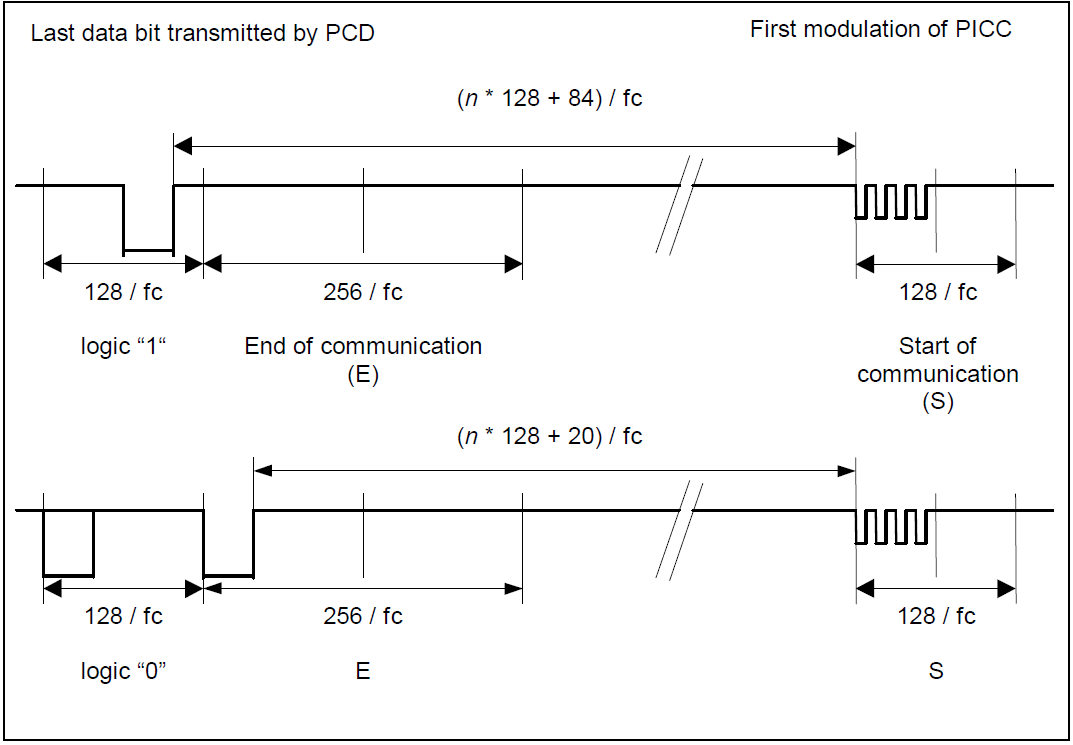
\includegraphics[width=6.1in,height=4.22in]{Norma_ISO/14443-3/media//image9.png}
        \end{center}
\end{figure}


%%%%%%%%%%%%%%%%%%%% Figure/Image No: 1 Ends here %%%%%%%%%%%%%%%%%%%%

\par
\begin{center}
Figura 3.7.6.1 - Demora temporal de trama PCD a PICC.
\end{center}
\par


\paragraph{Tiempo de retardo trama PICC a PCD}
Este es el tiempo transcurrido entre la última modulación transmitida por el PICC y la primera pausa transmitida por el PCD y deberá ser al menos 1172 / fc.\par

\paragraph{Tiempo de guardia de solicitud}
El Tiempo de guardia de solicitud se define como el tiempo mínimo entre los bits de inicio de dos comandos REQUEST consecutivos. Eso tiene el valor 7000 / fc.\par

\paragraph{Formatos de trama}
Los siguientes tipos de tramas se definen para el protocolo de detección de colisiones de bits.\par

\paragraph{Tramas REQA y WAKE-UP}
Las tramas de solicitud (REQA) y activación (WAKE-UP) se utilizan para iniciar la comunicación y consisten en, en el siguiente orden:\par

\begin{itemize}
	\item Inicio de comunicación\par

	\item 7 bits de datos transmitidos LSB primero. (El contenido de los datos es '26' para un REQA estándar y '52' para una solicitud de WAKE-UP).\par

	\item Fin de la comunicación
\end{itemize}\par

No se agrega bit de paridad.\par

%%%%%%%%%%%%%%%%%%%% Figure/Image No: 2 starts here %%%%%%%%%%%%%%%%%%%%
\begin{figure}[H]
	\begin{center}
		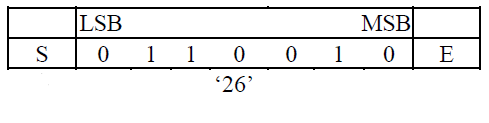
\includegraphics[width=3.76in,height=0.95in]{Norma_ISO/14443-3/media/image6.png}
        \end{center}
\end{figure}
%%%%%%%%%%%%%%%%%%%% Figure/Image No: 2 Ends here %%%%%%%%%%%%%%%%%%%%

\par
\begin{center}
Figura 3.7.6.2 -Tramas REQA y WAKE-UP.
\end{center}
\par

\par
\paragraph{Trama estándar}
Las tramas estándar se utilizan para el intercambio de datos y consisten en,\par

\begin{itemize}
	\item Inicio de comunicación\par

	\item N $\ast$  (8 bits de datos + bit de paridad impar). El LSB de cada byte de datos se transmite primero. Cada byte de datos es seguido por un bit de paridad impar.\par

	\item Fin de la comunicación
\end{itemize}\par

\paragraph{Marco de anticolisión orientado a bits}
Se detecta una colisión cuando al menos dos PICC transmiten patrones de bits diferentes a la PCD. En este caso, la portadora se modula con la subportadora durante toda la duración del bit para al menos un bit.\par

Las tramas de anticolisión orientadas a bits solo se utilizan durante los ciclos anticolisión de tramas de bits y son, de hecho, tramas estándar con una longitud de 7 bytes de datos, divididos en dos partes: parte 1 para transmisión de PCD a PICC y parte 2 para transmisión desde PICC a PCD.\par

Para la duración de la parte 1 y parte 2, se aplicarán las siguientes reglas:\par

Regla 1: La suma de los bits de datos será 56\par

Regla 2: la longitud mínima de la parte 1 será de 16 bits de datos\par

Regla 3: la longitud máxima de la parte 1 será de 55 bits de datos\par

En consecuencia, la longitud mínima de la parte 2 será de 1 bit de datos y la longitud máxima será de 40 bits de datos.\par

Como la división puede ocurrir en cualquier posición de bit dentro de un byte de datos, se definen dos casos:\par

Caso FULL BYTE: división después de un byte de datos completo. Se agrega un bit de paridad después del último bit de datos de la parte 1.\par

Caso SPLIT BYTE: división dentro de un byte de datos. No se agrega ningún bit de paridad después del último bit de datos de part1.\par

\paragraph{CRC\_A}
El proceso de codificación y verificación CRC\_A se define en la recomendación UIT-T V.41, párrafo 2. El polinomio generador utilizado para generar los bits de verificación es x $ \string^ $  16 + x $ \string^ $  12 + x $ \string^ $  5 + 1. El valor inicial será ' 6363 '. El CRC\_A se adjuntará a los bytes de datos y se transmitirá a través de tramas estándar.\par

\paragraph{Estados del PICC.}
Las siguientes secciones proporcionan descripciones de los estados para un PICC de tipo A específico del protocolo de detección de colisiones de bits.\par



%%%%%%%%%%%%%%%%%%%% Figure/Image No: 3 starts here %%%%%%%%%%%%%%%%%%%%

\begin{figure}[H]
	\begin{center}
		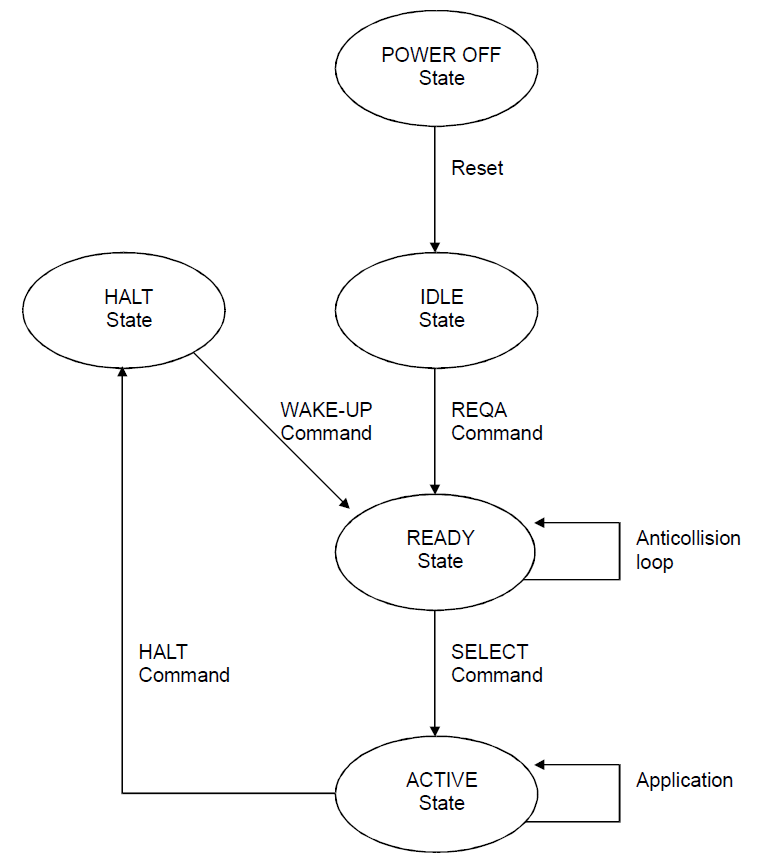
\includegraphics[width=6.27in,height=7.01in]{Norma_ISO/14443-3/media/image7.png}
        \end{center}
\end{figure}


%%%%%%%%%%%%%%%%%%%% Figure/Image No: 3 Ends here %%%%%%%%%%%%%%%%%%%%

\par

\par
\begin{center}
Figura 3.7.6.3 - Diagrama de estados PICC Tipo $``$A$"$ 
\end{center}
\par

\paragraph{Estado OFF}
En el estado de OFF, el PICC no recibe energía debido a la falta de energía del portador y no debe emitir subportadora.\par

\paragraph{Estado IDLE}
Después de que el campo haya estado activo durante un retraso máximo definido en la cláusula 5, el PICC ingresará en su estado IDLE. En este estado, el PICC está encendido, y es capaz de demodular y reconocer los comandos válidos de REQA y WAKE-UP del PCD.\par

\paragraph{Estado READY}
Este estado se ingresa tan pronto como se recibe y sale un mensaje REQA o WAKE-UP válido cuando el PICC está seleccionado con su UID. En este estado, se puede aplicar la anticolisión de la trama de bits u otro método anticolisión opcional. Los niveles de cascada se manejan dentro de este estado para obtener todo el UID CLn.\par

\paragraph{Estado ACTIVE}
Este estado se ingresa seleccionando el PICC con su UID completo.\par

\paragraph{Estado HALT}
Este estado se ingresa mediante el comando HALT definido en 3.7.6.3.4 o mediante un comando específico de la aplicación no definido en esta parte de ISO / IEC 14443. En este estado, un PICC responderá solo a un comando de WAKE-UP, que transita el PICC a su estado READY.\par

\paragraph{Conjunto de comandos}
Los comandos utilizados por el PCD para gestionar la comunicación con varios PICC son:\par

\begin{itemize}
	\item REQA\par

	\item WAKE-UP\par

	\item ANTICOLLISION\par

	\item SELECT\par

	\item HALT
\end{itemize}\par

Los comandos usan los formatos de byte y marco descriptos anteriormente.\par

\paragraph{Comando REQA}
El comando REQA es enviado por el PCD para sondear el campo de los PICC de tipo A.\par

\paragraph{Comando WAKE-UP}
El PCD envía el comando WAKE-UP para poner los PICC que han ingresado al estado HALT de nuevo en el estado READY. Luego, participarán en nuevos procedimientos de anticolisión y selección.\par

\paragraph{Comandos ANTICOLLISION y SELECT}
Estos comandos se usan durante un ciclo anticolisión. Los comandos ANTICOLLISION y SELECT constan de:\par

\begin{itemize}
	\item Seleccionar código SEL (1 byte)\par

	\item Número de bits válidos NVB (1 byte)\par

	\item De 0 a 40 bits de datos de UID CLn según el valor de NVB
\end{itemize}\par

SEL especifica el nivel de cascada CLn.\par

NVB especifica el número de bits válidos de UID CLn transmitidos por el PCD.\par

\paragraph{Comando HALT}
El comando HALT consta de cuatro bytes y se transmitirá utilizando la trama estándar.\par



%%%%%%%%%%%%%%%%%%%% Figure/Image No: 4 starts here %%%%%%%%%%%%%%%%%%%%

\begin{figure}[H]
	\begin{center}
		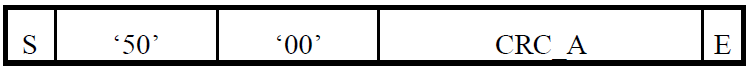
\includegraphics[width=5.47in,height=0.51in]{Norma_ISO/14443-3/media/image10.png}
        \end{center}
\end{figure}


%%%%%%%%%%%%%%%%%%%% Figure/Image No: 4 Ends here %%%%%%%%%%%%%%%%%%%%

\par
\begin{center}
Figura 3.7.6.4 - Trama del comando HALT.
\end{center}
\par

Si el PICC responde con cualquier modulación durante un período de 1 ms después del final de la trama HALT, esta respuesta se interpretará como "no reconocido".\par

\paragraph{Secuencia SELECT}
El propósito de esta secuencia es el de obtener el UID de un PICC y seleccionar a este PICC para una futura comunicación.\par

\paragraph{ATQA - Respuesta al comando REQA}
Después de que el PCD transmite el comando REQA, todos los PICC responden de forma síncrona con su respuesta (ATQA), que codifica el tipo anticolisión aplicable en dos bytes de datos.\par

Si hay múltiples respuestas PICC, pueden producirse colisiones. El PCD decodificará una colisión dentro de ATQA. Esto da como resultado un OR lógico de todos los ATQA.\par

\paragraph{Anticolisión y selección}
\paragraph{Bucle anticolisión dentro de cada nivel de cascada}
El siguiente algoritmo se aplicará al ciclo anticolisión:\par

\begin{itemize}
	\item Paso 1: El PCD asigna SEL con el código para el tipo de anticolisión seleccionado y el nivel de cascada.\par

	\item Paso 2: El PCD asigna NVB con el valor de '20'.\par

	\item Paso 3: El PCD transmite SEL y NVB.\par

	\item Paso 4: Todos los PICC en el campo responderán con su UID CLn completa.\par

	\item Paso 5: Suponiendo que los PICC en el campo tengan números de serie únicos, entonces, si responde más de un PICC, se produce una colisión. Si no ocurre una colisión, se omiten los pasos 6 a 10.\par

	\item Paso 6: El PCD reconocerá la posición de la primera colisión.\par

	\item Paso 7: El PCD asigna NVB con un valor que especifica el número de bits válidos de UID CLn. Los bits válidos serán parte del UID CLn que se recibió antes de que ocurriera una colisión añadida por un (0) by (1) b, decidido por el PCD. Una implementación típica agrega a (1) b.\par

	\item Paso 8: El PCD transmite SEL y NVB, seguidos de los bits válidos.\par

	\item Paso 9: Solo los PICC cuya parte de UID CLn es igual a los bits válidos transmitidos por el PCD transmitirán sus bits restantes del UID CLn.\par

	\item Paso 10: Si ocurren más colisiones, se repiten los pasos 6 a 9. La cantidad máxima de bucles será 32.\par

	\item Paso 11: Si no hay más colisiones, la PCD asigna NVB con el valor de '70'.\par

	\item Paso 12: El PCD transmite SEL y NVB, seguidos de los 40 bits de UID CLn, seguidos por CRC\_A suma de comprobación.\par

	\item Paso 13: El PICC que UID CLn coincide con los 40 bits responde con su SAK.\par

	\item Paso 14: Si el UID está completo, el PICC transmitirá SAK con un bit en cascada despejado y el tránsito desde el estado LISTO al estado ACTIVO.\par

	\item Paso 15: El PCD verificará si el bit en cascada de SAK está configurado para decidir si seguirán ciclos de anticolisión adicionales con un nivel de cascada incrementado.
\end{itemize}\par

Si el UID de un PICC es conocido, el PCD puede omitir el paso 2 al paso 10 para seleccionar este PICC sin realizar el ciclo anticolisión.\par

\paragraph{Código de SEL}
Longitud: 1 byte\par

Valores posibles: '93', '95', '97'.\par

\paragraph{Código de NVB (número de bits válidos)}
Longitud: 1 byte\par

Los 4 bits superiores se llaman por cuenta y especifican el número de todos los bits de datos válidos divididos entre 8, incluidos SEL y NVB transmitidos por el PCD. En consecuencia, el valor mínimo de bytecount es 2 y el valor máximo es 7.\par

Los 4 bits más bajos se denominan bitcount y especifican el número de todos los bits de datos válidos módulo 8 transmitidos por el PCD.\par

\paragraph{Código de SAK}
SAK es transmitido por el PICC cuando NVB ha especificado 40 bits de datos válidos y cuando todos estos bits de datos coinciden con UID CLn.\par

SAK se transmite a través la trama estándar, seguido de CRC\_A.\par

Si el UID no está completo, el PICC permanecerá en estado READY y el PCD iniciará un nuevo ciclo de anticolisión con un nivel de cascada incrementado.\par

Si el UID está completo, el PICC transmitirá SAK con el bit de cascada despejado y el tránsito del estado READY al estado ACTIVE. El PICC configurará el bit b6 de SAK cuando haya información adicional disponible.\par

La definición de la información adicional no está sujeta a esta parte del estándar y se definirá en ISO / IEC 14443-4.\par

\paragraph{Contenido de UID y niveles de cascada}
El UID consta de 4, 7 o 10 bytes UID. En consecuencia, el PICC manejará hasta 3 niveles de cascada para obtener todos los bytes de UID.\par

Dentro de cada nivel de cascada, una parte del UID que consta de 5 bytes de datos se transmitirá a la PCD. De acuerdo con la nivel de cascada máximo, se definen tres tipos de tamaño de UID. Este tamaño de UID debe ser consistente con la tabla 6.4.\par



%%%%%%%%%%%%%%%%%%%% Figure/Image No: 5 starts here %%%%%%%%%%%%%%%%%%%%

\begin{figure}[H]
	\begin{center}
		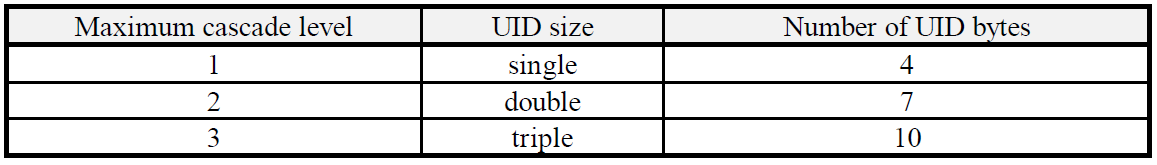
\includegraphics[width=6.27in,height=0.89in]{Norma_ISO/14443-3/media/image8.png}
        \end{center}
\end{figure}


%%%%%%%%%%%%%%%%%%%% Figure/Image No: 5 Ends here %%%%%%%%%%%%%%%%%%%%

\par
\begin{center}
Figura 3.7.6.4 - Tamaños de los UID.
\end{center}
\par